\documentclass[aspectratio=169]{beamer}

\usetheme{default}
\setbeamertemplate{navigation symbols}{}
\setbeamertemplate{itemize item}{\color{black}\textbullet}
\setbeamertemplate{itemize subitem}{\color{black}\textbullet}
\usepackage{xcolor}
\definecolor{navy}{RGB}{0, 0, 128}
\definecolor{lightblue}{RGB}{230,240,250}
\definecolor{darkgreen}{RGB}{0,100,0}
\definecolor{lightgreen}{RGB}{230,250,230}
\newcommand{\highlight}[1]{\colorbox{lightblue}{$\displaystyle\textcolor{navy}{#1}$}}
\newcommand{\highlighttext}[1]{\colorbox{lightblue}{\textcolor{navy}{#1}}}
\newcommand{\highlightgreen}[1]{\colorbox{lightgreen}{$\displaystyle\textcolor{darkgreen}{#1}$}}

\begin{document}

\begin{frame}
\centering
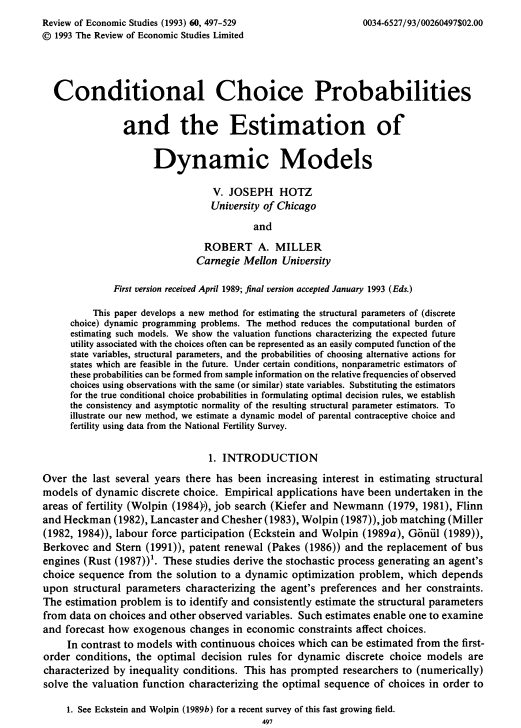
\includegraphics[width=.42\textwidth]{HotzMiller_cover.jpg}
\end{frame}



\begin{frame}

Hotz-Miller inversion proposition: 
\bigskip\par

There exists an invertible mapping $\psi$ from CCPs ($p$'s) to $(v_j - v_k)$'s

\begin{align*}
V_{t+1}&= v_{0t+1} + \mathbb{E}\max\{\epsilon_{0t+1}, \highlight{v_{1t+1} - v_{0t+1}} + \epsilon_{1t+1}, \ldots, \highlightgreen{v_{Jt+1} - v_{0t+1}} + \epsilon_{Jt+1}\}\\[1.5em]
&= v_{0t+1} + \mathbb{E}\max\{\epsilon_{0t+1}, \highlight{\psi_0^1(p_{t+1})} + \epsilon_{1t+1}, \ldots, \highlightgreen{\psi_0^J(p_{t+1})} + \epsilon_{Jt+1}\}
\end{align*}

\end{frame}



\begin{frame}
The $p$'s come from data, but we need:
\bigskip\par
\begin{itemize}
\itemsep1.5em
\item<2-> The mapping $\psi\left(\cdot\right)$
\item<3-> To calculate expectations of $\epsilon$'s
\item<4-> To handle the $v_{0t+1}$'s
\end{itemize}

\onslide<5->{
\bigskip\par
Now let's go through an example with $\mathcal{J}=\{0,1\}$ and stochastic $X$'s
}

\onslide<6->{
\bigskip\par
Suppose option 0 is a \textcolor{navy}{terminal choice}---no further choices after choosing 0
}


\end{frame}



\begin{frame}

How can we simplify the conditional value function $v_{1t}$ in this setting?

\only<1>{
\begin{align*}
v_{1t}(X_t) &= u_1(X_t) + \beta\sum_{X_{t+1}}V_{t+1}(X_{t+1})f_1(X_{t+1}|X_t)
&\\
&\phantom{= u_1(X_t) + \beta\sum_{X_{t+1}}\Big[v_{0t+1}(X_{t+1}) + \mathbb{E}\max\{\epsilon_{0t+1}, \psi_0^1(p_{t+1}) + \epsilon_{1t+1}\}\Big]f_1(X_{t+1}|X_t)}
\end{align*}
}

\only<2->{
\begin{align*}
v_{1t}(X_t) &= u_1(X_t) + \beta\sum_{X_{t+1}}V_{t+1}(X_{t+1})f_1(X_{t+1}|X_t)\\
&\\
&= u_1(X_t) + \beta\sum_{X_{t+1}}\Big[v_{0t+1}(X_{t+1}) + \mathbb{E}\max\{\epsilon_{0t+1}, \psi_0^1\left(p(X_{t+1})\right) + \epsilon_{1t+1}\}\Big]f_1(X_{t+1}|X_t)
\end{align*}
}

\onslide<3->{
\bigskip{}
If $v_{0t+1}(X_{t+1}) = X_{t+1}\alpha_0$, no backwards recursion needed
}

\onslide<4->{
\bigskip{}
... so long as we can handle the expectation term
}

\end{frame}







\begin{frame}

\onslide<1->{
With T1EV errors:
\begin{align*}
\mathbb{E}\max\{\epsilon_{0t+1}, \psi_0^1\left(p(X_{t+1})\right) + \epsilon_{1t+1}\} &= - \log\left(p_0(X_{t+1})\right)+c
\end{align*}
}
\onslide<2>{
How?
}

\onslide<3->{
How? We showed before that $V_{t+1} = v_{jt+1}-\log\left(p_{jt+1}\right)+c$ for any $j$ when $\epsilon\sim$T1EV
\bigskip\par
}

\onslide<4->{
Therefore:
\begin{align*}
v_1(X_t) &= u_1(X_t) + \beta\sum_{X_{t+1}}\Big[v_{0t+1}(X_{t+1}) + \underbrace{\mathbb{E}\max\{\epsilon_{0t+1}, \psi_0^1\left(p(X_{t+1})\right) + \epsilon_{1t+1}\}}_{-\log\left(p_0(X_{t+1})\right)+c}\Big]f_1(X_{t+1}|X_t)
\end{align*}
}
\onslide<5->{
Expressed as function of CCPs:
\begin{align*}
v_{1t}(X_t) = u_1(X_t) + \beta\sum_{X_{t+1}}\Big[v_{0t+1}(X_{t+1}) - \log(p_0(X_{t+1}))\Big]f_1(X_{t+1}|X_t) + \beta c
\end{align*}
}

\end{frame}

\begin{frame}

Implementation steps when choice 0 is terminal:
\bigskip\par

\begin{itemize}
\itemsep1.5em
\item<1-> $v_{0t+1}$ is linear in parameters (i.e., no $V_{t+2}$ recursion)
\item<2-> Estimate $p_0(X_{t+1})$ from data (e.g., bin estimator)
\item<3-> Similar to first-stage estimation of $f_j(X_{t+1}|X_t)$
\item<4-> Problem reduces to logit with adjustment term for $\log(p_{0t+1})$
\item<4->[]
\begin{itemize}
\itemsep1.5em
    \item<5-> Stage 1: estimate $p$'s and $f$'s via bin estimator
    \item<6-> Stage 2: estimate $\alpha$'s via logit with constructed adjustment term
\end{itemize}
\end{itemize}
\end{frame}


\begin{frame}

Hotz-Miller application: Couples' fertility and sterilization decisions
\bigskip\par

\begin{itemize}
\itemsep1.5em
\item<2-> State: $H_t$ = number of children, wife's age, wife's education
\item<3-> Choices: $j=0$ (sterilize), $j=1$ (no sterilization)
\item<4-> Sterilization is \textcolor{navy}{terminal}---no further fertility decisions
\item<5-> If no sterilization: probability $\alpha$ of birth next period
\end{itemize}

\onslide<6->{
\bigskip\par
e.g.
$f_1(H_{t+1}\vert H_t) = \alpha\cdot 1[H_{t+1}=H_t+1] + (1-\alpha)\cdot 1[(H_{t+1}=H_t)]$
}

\end{frame}





\end{document}